\section{介绍}
\qquad
在一个电路板上,给定一个均匀分布的$n\times n$个内部节点,要求确定电路板的大小,计算各个节点到电路板边界的路径,使得各个路径不相交并且长度之和最短。

为了解决这个问题,本项目实现了基于费用流的布线方案,该方案能够获得最优解,然而由于不适应与大规模的数据,因此又实现了基于规则的布线方案,该方案可以在可以接受的时间内得到较优的解。关于具体的实现算法见第 \ref{algo} 节,具体的设计思路见第 \ref{sys-arch} 节。

我们支持将计算得到的方案以图片形式输出到文件或窗口,同时也支持以原始路径的形式保存到文件。并且支持从文件中读取原始数据并且显示到窗口。

目前为止,我们基于规则的算法最大支持$150\times 150$个节点。

\begin{figure}[htpb]
	\centering
	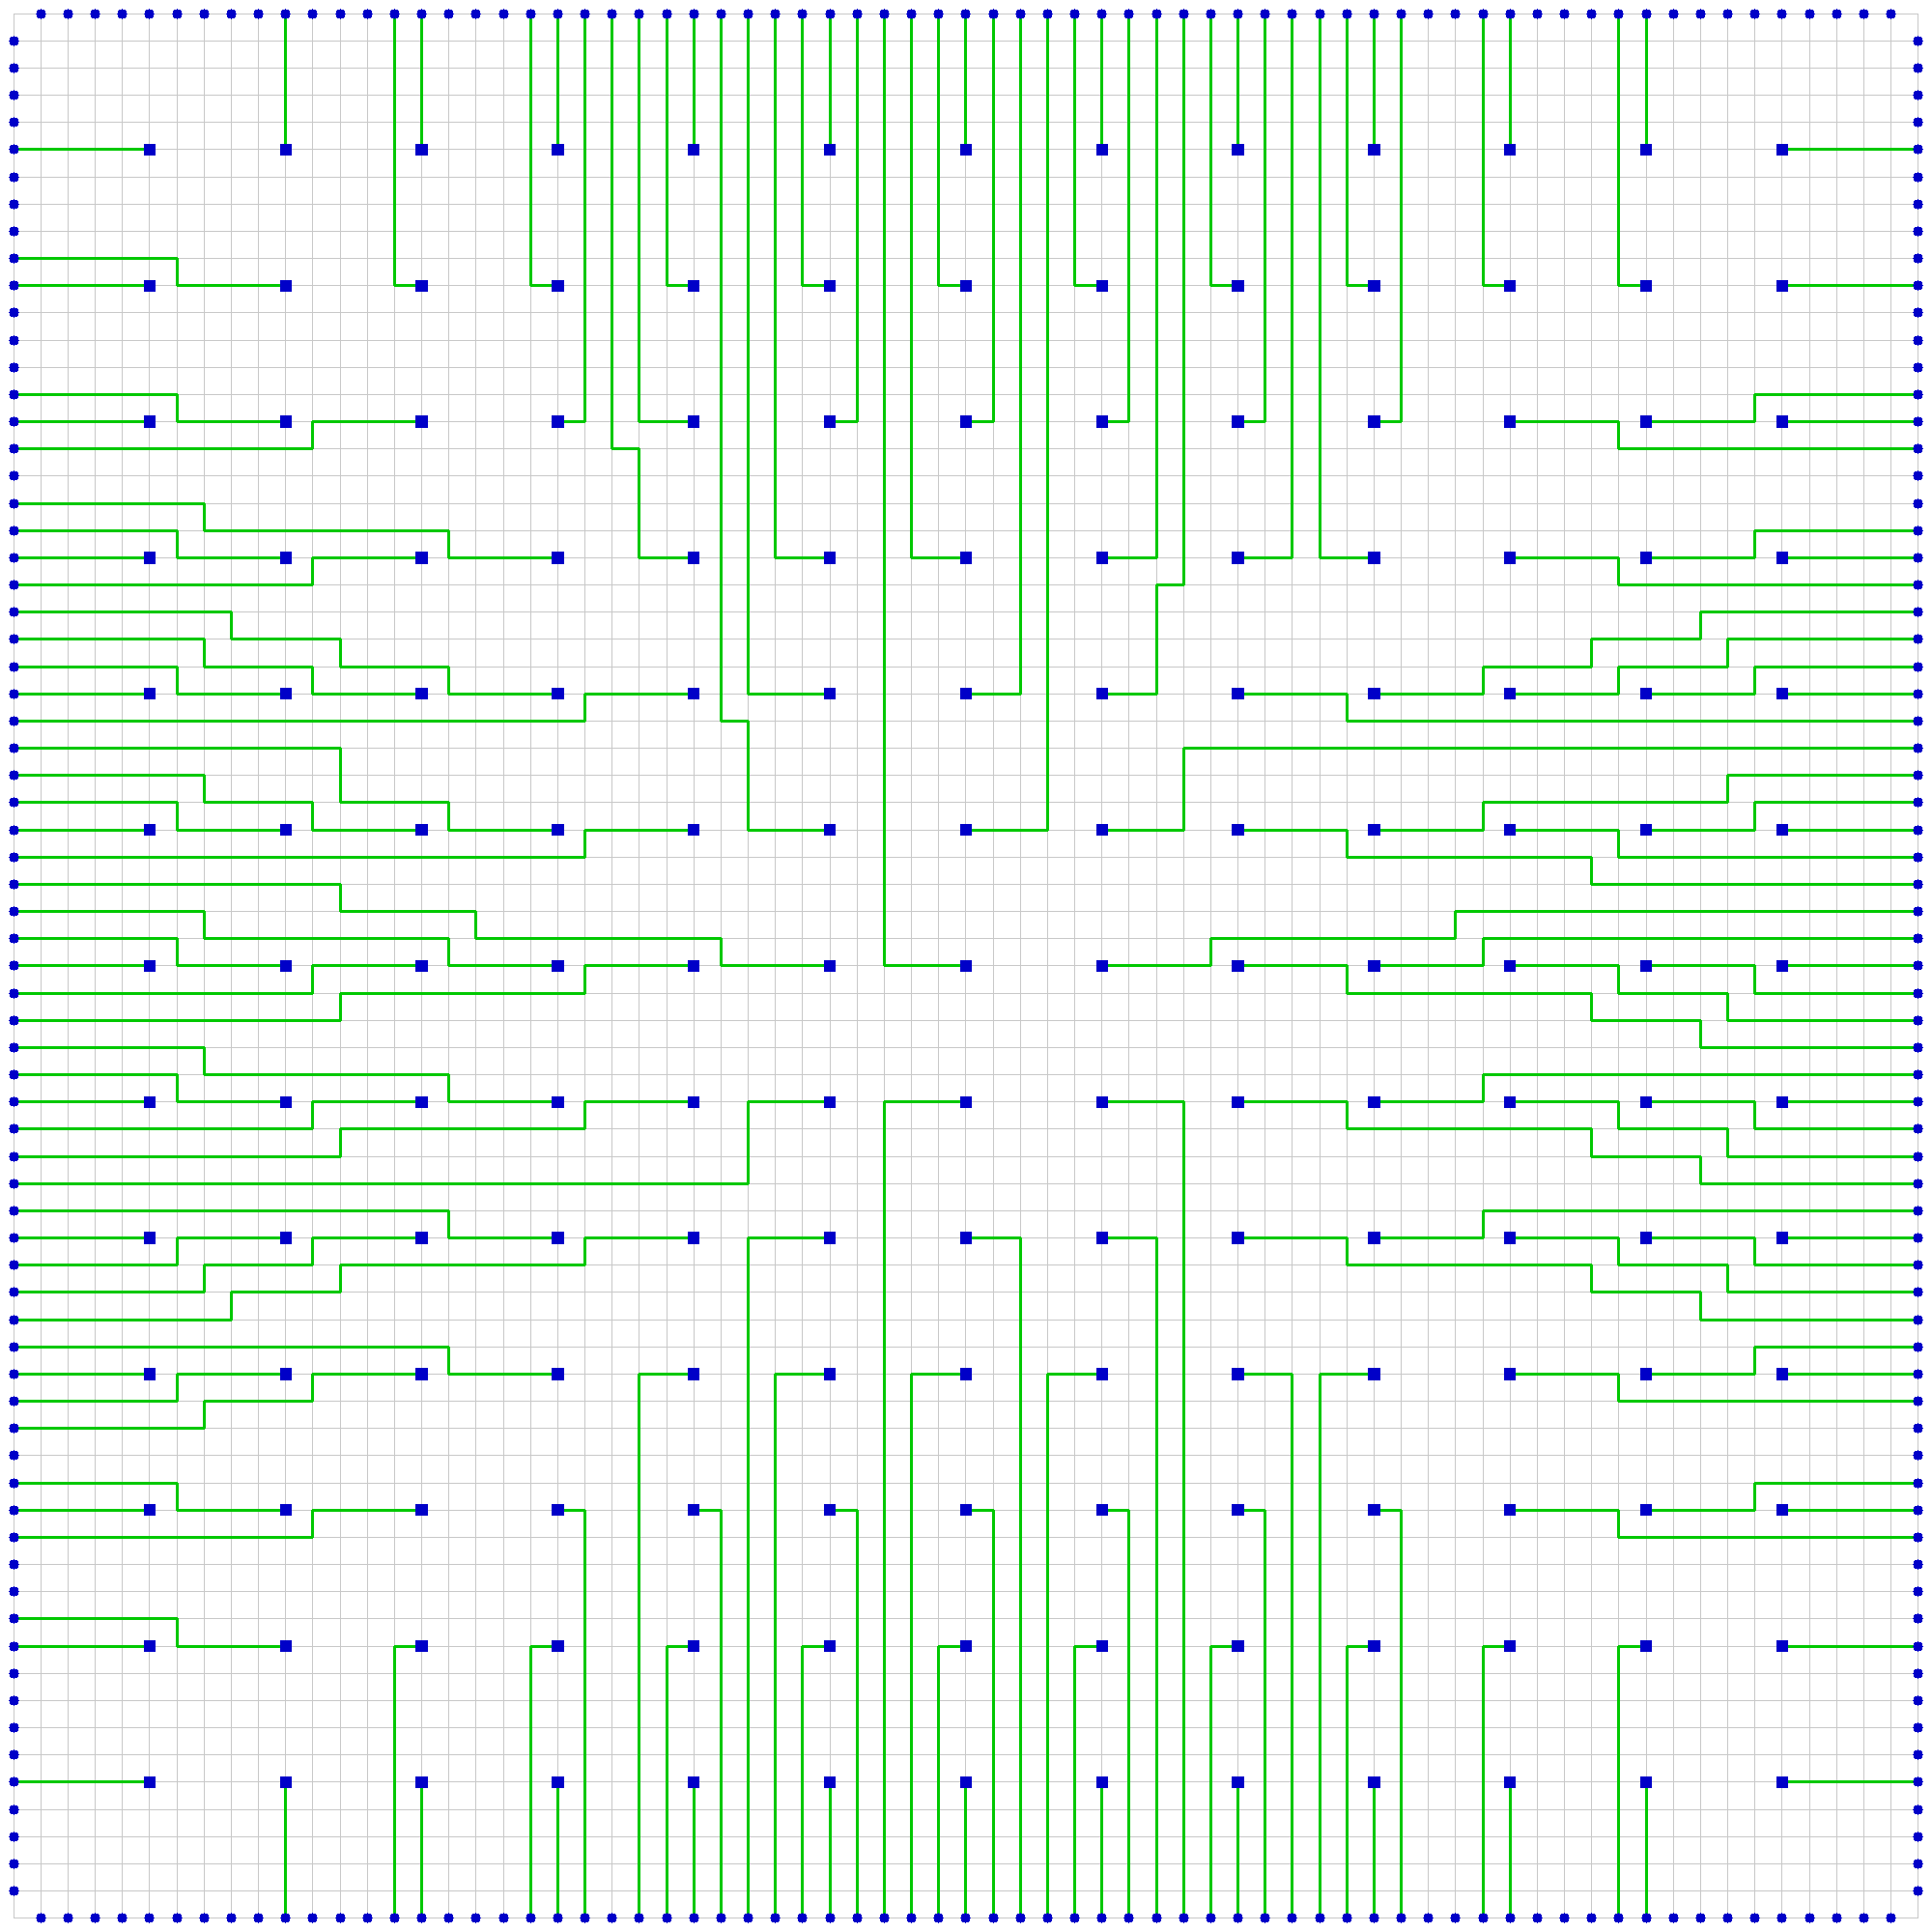
\includegraphics[height=2in]{../testcase/small-cases/13x13-71x71.png}
	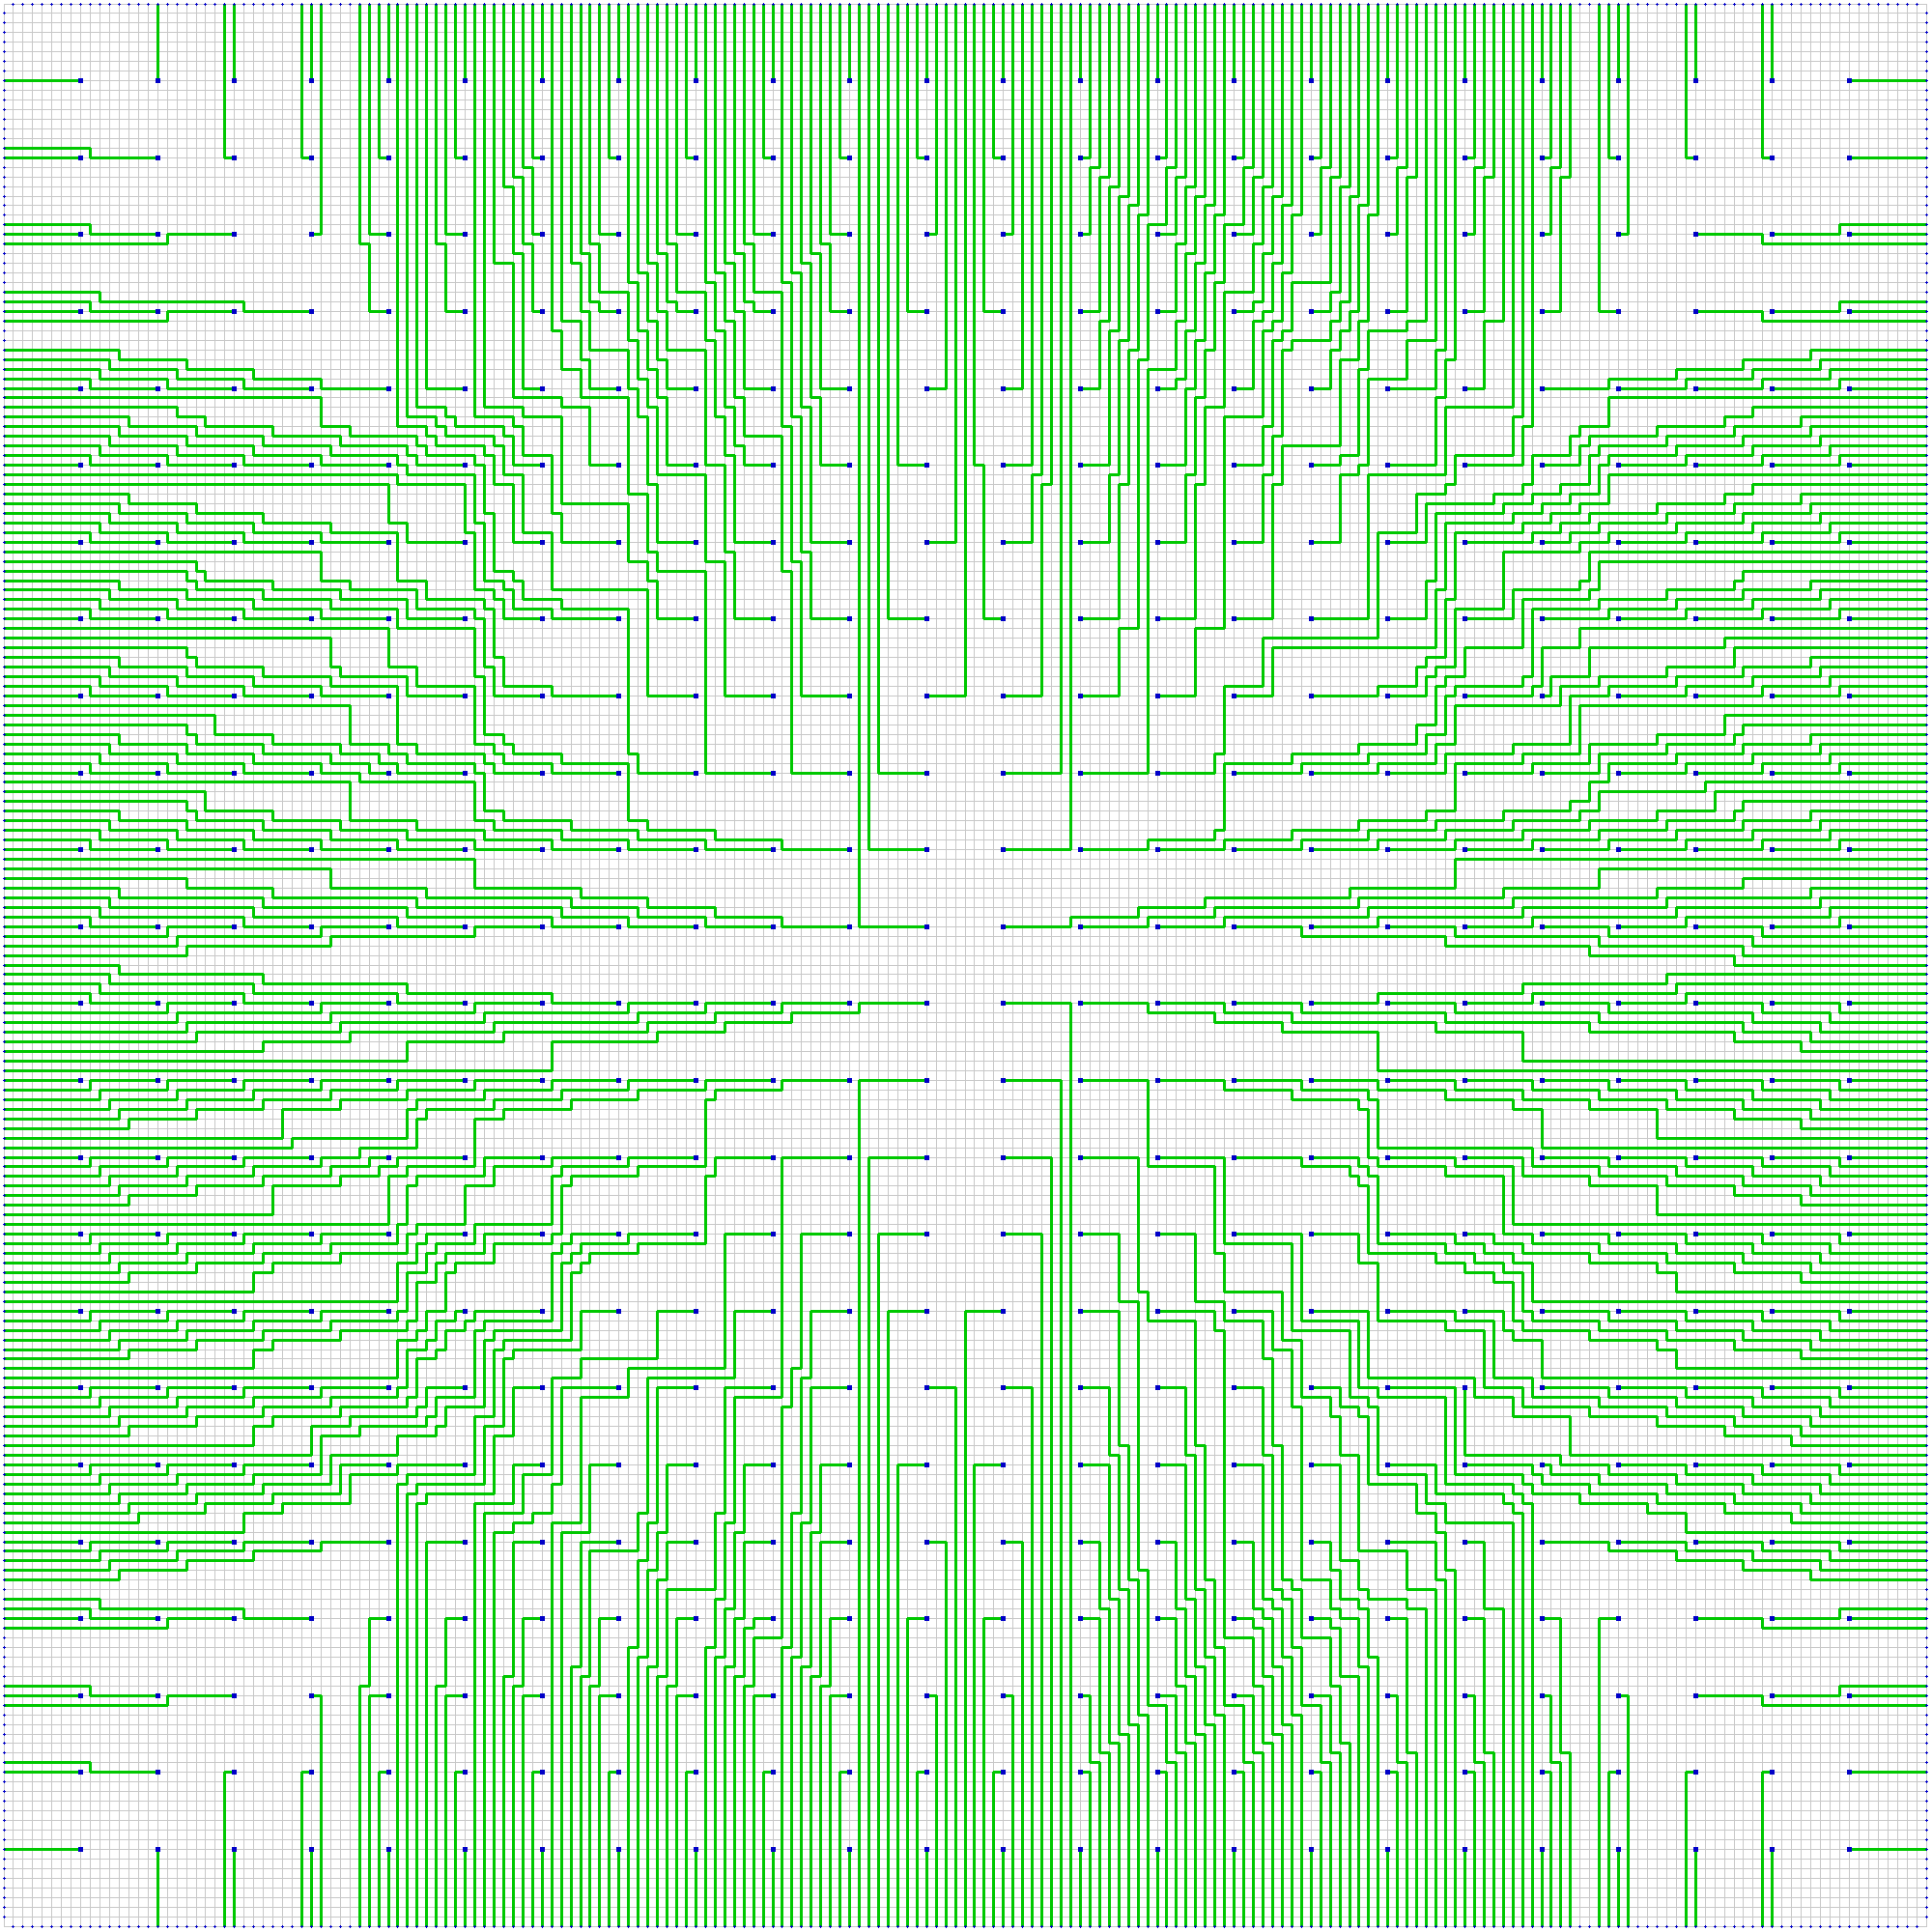
\includegraphics[height=2in]{../testcase/small-cases/24x24-201x201.png}
	\caption{两个基于网络流方案的例子}
\end{figure}
